\section{Data}
In Section \ref{cont_vol} wee looked into the assumption of constant volatility in the Black Scholes model. 
Where during the study, a 10Y10Y EUR swaption was introduced. This chapter will provide a introduction to 
market data on swaption. In this thesis the data source is Citi Velocity, which is a market data plantformed
owned by Citi Bank.
\\\\
Before delving into the market data on swaptions, let's revisit the definition of a swaption. 
A swaption gives the holder the right, but not the obligation, to enter into an interest rate swap in the future. 
There are two types of swaptions: payer swaptions and receiver swaptions, as previously described.
\\\\
The four main parameters defining a swaption are:
\begin{itemize}
\item \textbf{Expiry} \quad when in the future the holder can exercise their right.
\item \textbf{Tenor} \quad  the maturity of the underlying interest rate swap.
\item \textbf{Strike} \quad the pre-specified interest rate of the swap.
\item \textbf{Pay/Receive} \quad whether the investor pays or receives the fixed rate.
\end{itemize}
\noindent
A 10Y10Y EUR swaption was analyzed, but let's clarify what a 10Y10Y EUR swaption entails. 
Assuming the swaption is a receiver swaption, it represents a contract that, in ten years, 
gives the holder the right to enter into a ten-year interest rate swap in EUR, receiving a fixed rate. 
Thus, the swaption has an expiry of 10 years, a tenor of 10 years, and a strike equivalent to the value of the fixed rate. 
It's important to note that the underlying interest rate swap in the swaption is a forward swap, commencing 10 years from now.
\\\\
Then before we will look at some the displayed data, lets first cover some lingo of swaption. 
A swaption with a strike set at the current market rate for the underlying forward swap is referred 
to as at-the-money-forward (ATMF). If the strike differs from the ATMF rate, the swaption is categorized as out-of-the-money (OTM).

\begin{table}[h]
    \centering
    \begin{tabular}{|c|c|c|c|c|c|c|c|c|c|}
     \hline  
     \multicolumn{10}{|c|}{Tenor} \\ 
    \hline
     Expiry& 1Y & 2Y & 3Y & 5Y & 7Y & 10Y & 15Y & 20Y & 30Y \\
    \hline
    1M & 5.2896 & 6.0865 & 5.9731 & 5.6770 & 5.4074 & 5.0402 & 4.8121 & 4.6578 & 4.5098 \\
    2M & 5.4361 & 6.1242 & 5.9983 & 5.7206 & 5.4838 & 5.1569 & 4.9592 & 4.7942 & 4.6228 \\
    3M & 5.5244 & 6.1032 & 5.9953 & 5.7530 & 5.5240 & 5.1959 & 5.0318 & 4.8662 & 4.6948 \\
    6M & 6.0007 & 6.3187 & 6.1810 & 5.9009 & 5.7098 & 5.4304 & 5.2822 & 5.1272 & 4.9696 \\
    9M & 6.2264 & 6.3990 & 6.2515 & 6.0103 & 5.8553 & 5.6185 & 5.4686 & 5.3155 & 5.1284 \\
    12M & 6.2698 & 6.3692 & 6.2157 & 6.0080 & 5.8713 & 5.6575 & 5.4984 & 3.5614 & 5.1749 \\
    18M & 6.3333 & 6.3395 & 6.2046 & 6.0073 & 5.8874 & 5.7166 & 5.5284 & 5.3998 & 5.2215 \\
    2Y & 6.2967 & 6.2853 & 6.1613 & 5.9773 & 5.8477 & 5.7289 & 5.5014 & 5.3854 & 5.2146 \\
    3Y & 6.1824 & 6.1546 & 6.0463 & 5.8606 & 5.7536 & 5.6654 & 5.4234 & 5.2916 & 5.1171 \\
    4Y & 6.0380 & 6.0008 & 5.8975 & 5.7407 & 5.6613 & 5.5681 & 5.3010 & 5.1479 & 4.9677 \\
    5Y & 5.8966 & 5.8683 & 5.7524 & 5.6119 & 5.5376 & 5.4563 & 5.1646 & 5.0015 & 4.8213 \\
    7Y & 5.6398 & 5.6152 & 5.5170 & 5.3796 & 5.2946 & 5.2228 & 4.9248 & 4.7421 & 4.5575 \\
    10Y & 5.3399 & 5.3311 & 5.2101 & 5.0614 & 4.9531 & 4.8315 & 4.5247 & 4.3559 & 4.1757 \\
    12Y & 5.1687 & 5.1598 & 5.0635 & 4.8726 & 4.7460 & 4.5879 & 4.2716 & 4.1312 & 3.9422 \\
    15Y & 4.9532 & 4.9412 & 4.8215 & 4.5966 & 4.4391 & 4.2880 & 3.9736 & 3.8382 & 3.6523 \\
    20Y & 4.5909 & 4.5840 & 4.4649 & 4.2116 & 4.0605 & 3.8790 & 3.5666 & 3.4626 & 3.2743 \\
    30Y & 4.1109 & 4.1065 & 3.9893 & 3.6882 & 3.5119 & 3.2952 & 3.0168 & 2.9317 & 2.7602 \\
    \hline
    \end{tabular}
    \caption{}
\end{table}
    

    

\begin{table}[H]
    \centering
    \begin{tabular}{|l|*{11}{c|}}
    \hline
        Expiry x Tenor & -200 & -100 & -75 & -50 & -25 & ATM & 25 & 50 & 75 & 100 & 200 \\
    \hline
    10Y x 1Y & 0.514 & 0.518 & 0.521 & 0.524 & 0.528 & 0.533 & 0.539 & 0.545 & 0.552 & 0.560 & 0.594 \\
    10Y x 2Y & 0.515 & 0.518 & 0.521 & 0.524 & 0.528 & 0.533 & 0.538 & 0.544 & 0.551 & 0.558 & 0.591 \\
    10Y x 3Y & 0.506 & 0.508 & 0.510 & 0.513 & 0.516 & 0.521 & 0.525 & 0.531 & 0.537 & 0.544 & 0.577 \\
    10Y x 5Y & 0.497 & 0.495 & 0.497 & 0.499 & 0.502 & 0.506 & 0.510 & 0.515 & 0.521 & 0.527 & 0.557 \\
    10Y x 7Y & 0.492 & 0.486 & 0.487 & 0.489 & 0.491 & 0.495 & 0.498 & 0.503 & 0.509 & 0.515 & 0.547 \\
    10Y x 10Y & 0.488 & 0.477 & 0.477 & 0.478 & 0.479 & 0.483 & 0.485 & 0.490 & 0.496 & 0.502 & 0.536 \\
    10Y x 12Y & 0.474 & 0.463 & 0.463 & 0.463 & 0.464 & 0.467 & 0.470 & 0.475 & 0.480 & 0.487 & 0.520 \\
    10Y x 15Y & 0.462 & 0.449 & 0.448 & 0.448 & 0.449 & 0.452 & 0.455 & 0.459 & 0.465 & 0.471 & 0.504 \\
    10Y x 20Y & 0.449 & 0.434 & 0.433 & 0.432 & 0.433 & 0.435 & 0.438 & 0.442 & 0.447 & 0.453 & 0.486 \\
    10Y x 30Y & 0.436 & 0.419 & 0.417 & 0.416 & 0.416 & 0.417 & 0.420 & 0.423 & 0.428 & 0.434 & 0.466 \\
    \hline
    \end{tabular}
    \caption{Out-of-the-money-forward (OTMF) swaption volatility surface. Data source Citi Velocity  from  21.02.2024. }
    \label{tab:swaption_skew_data_2024}
\end{table}

\begin{figure}[H]
    \centering
    \begin{minipage}{0.5\textwidth}
        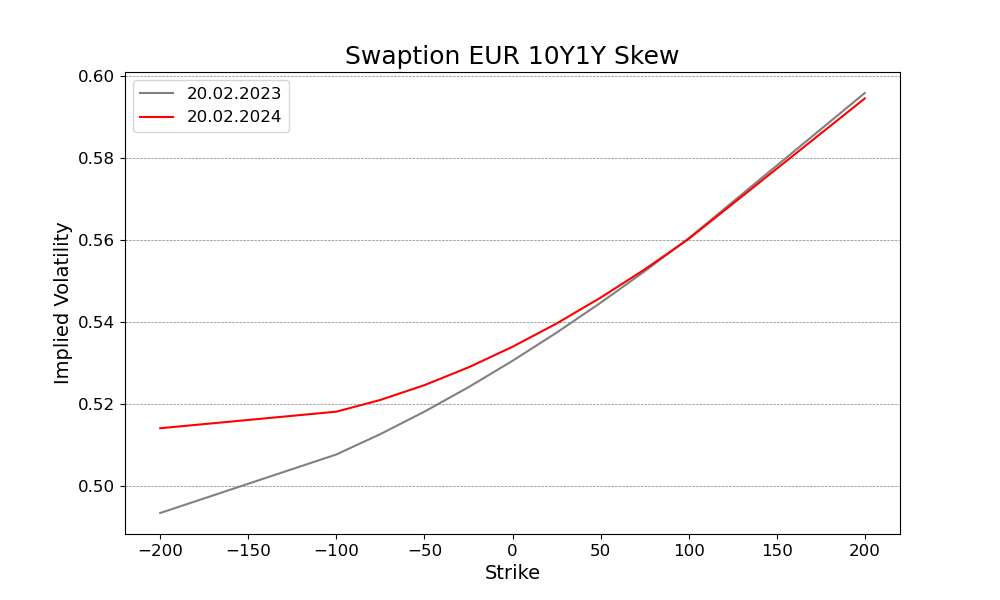
\includegraphics[width=\linewidth]{/Users/nannaingemannohrt/Desktop/master_thesis/main/plots/10Y1Y.png}
        \caption{EUR swaption 10Y1Y}
        \label{fig:10Y1Y}
    \end{minipage}\hfill 
    \begin{minipage}{0.5\textwidth}
        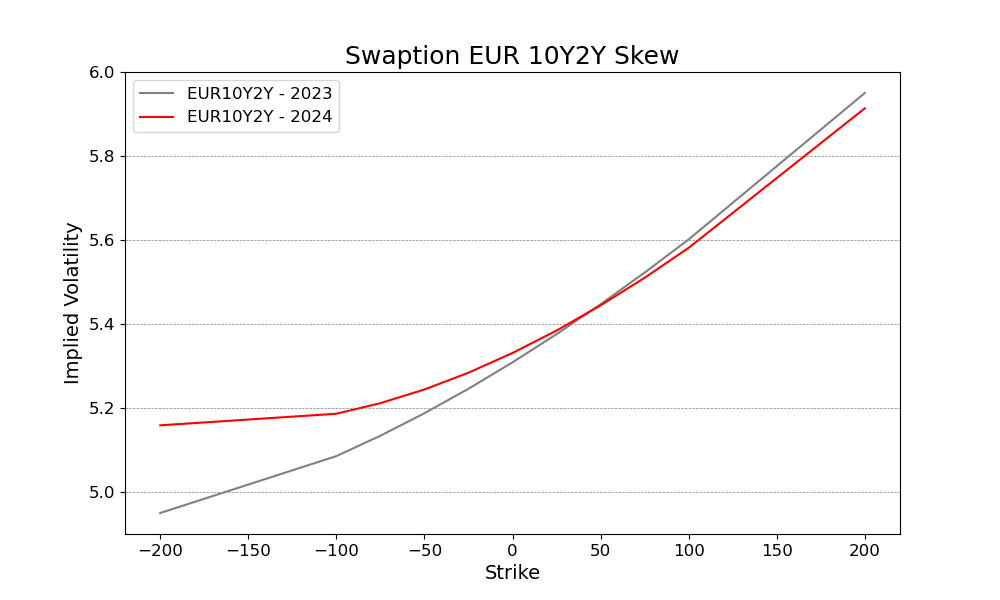
\includegraphics[width=\linewidth]{/Users/nannaingemannohrt/Desktop/master_thesis/main/plots/10Y2Y.png}
        \caption{EUR swaption 10Y2Y}
        \label{fig:10Y2Y}
    \end{minipage}

    \centering
    \begin{minipage}{0.5\textwidth}
        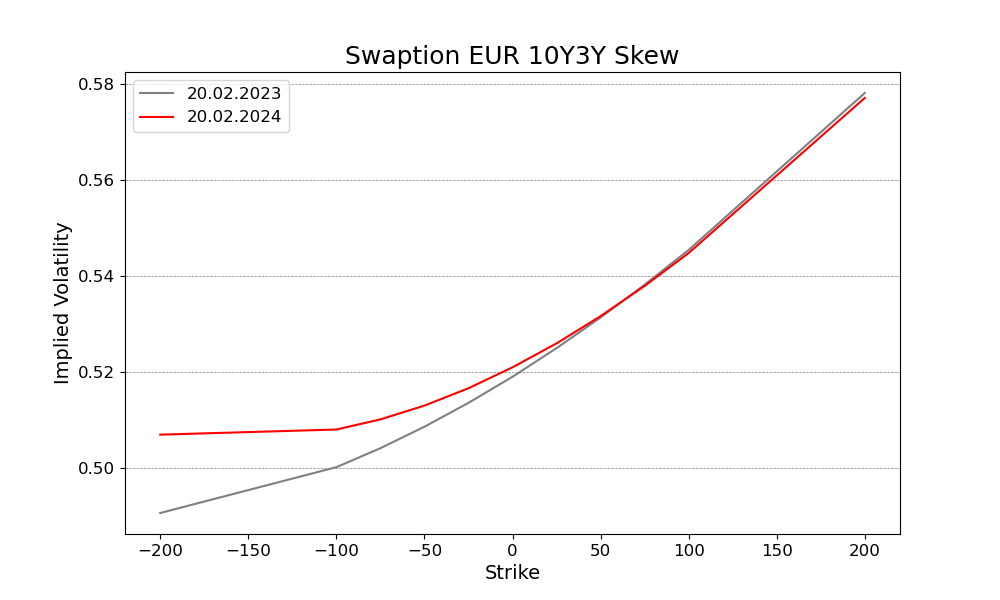
\includegraphics[width=\linewidth]{/Users/nannaingemannohrt/Desktop/master_thesis/main/plots/10Y3Y.png}
        \caption{EUR swaption 10Y3Y}
        \label{fig:10Y3Y}
    \end{minipage}\hfill 
    \begin{minipage}{0.5\textwidth}
        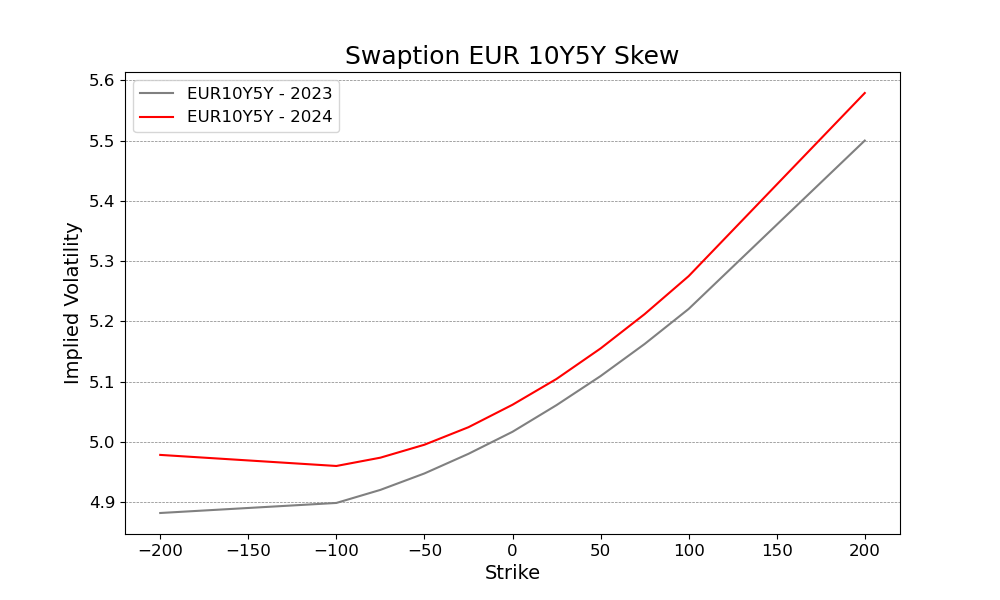
\includegraphics[width=\linewidth]{/Users/nannaingemannohrt/Desktop/master_thesis/main/plots/10Y5Y.png}
        \caption{EUR swaption 10Y5Y}
        \label{fig:10Y5Y}
    \end{minipage}

    \centering
    \begin{minipage}{0.5\textwidth}
        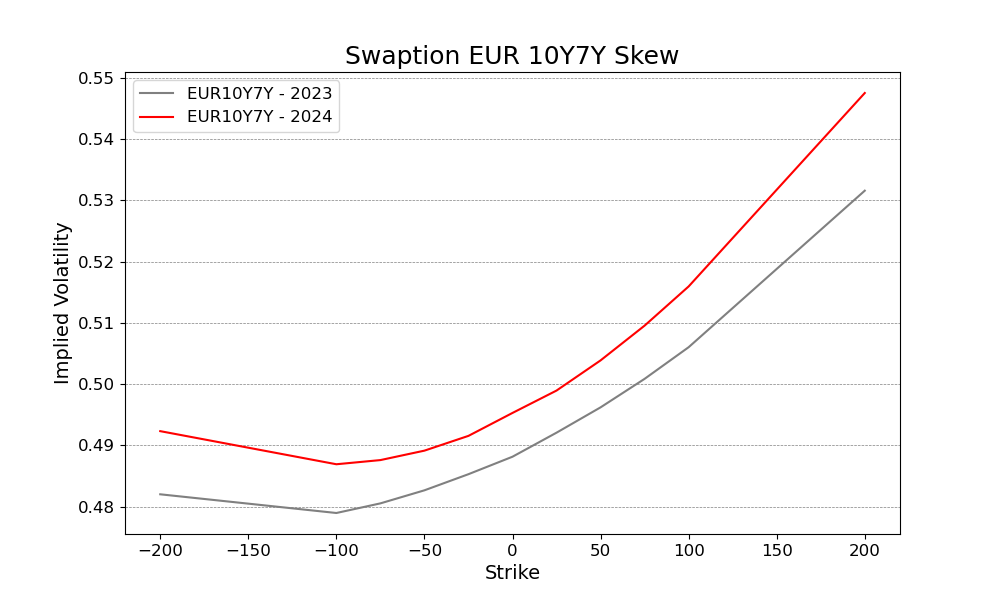
\includegraphics[width=\linewidth]{/Users/nannaingemannohrt/Desktop/master_thesis/main/plots/10Y7Y.png}
        \caption{EUR swaption 10Y7Y}
        \label{fig:10Y7Y}
    \end{minipage}\hfill 
    \begin{minipage}{0.5\textwidth}
        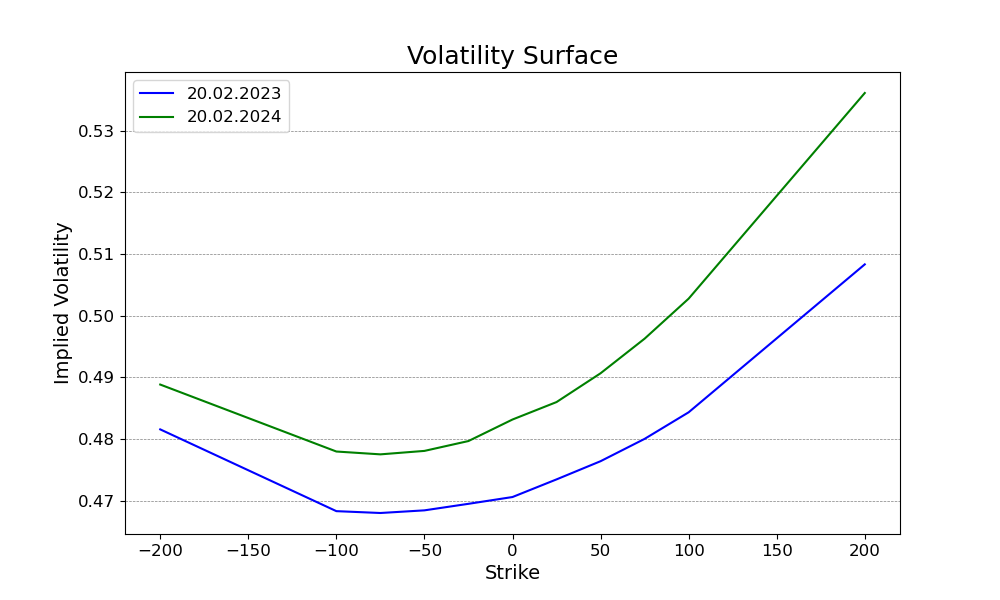
\includegraphics[width=\linewidth]{/Users/nannaingemannohrt/Desktop/master_thesis/main/plots/10Y10Y.png}
        \caption{EUR swaption 10Y10Y}
        \label{fig:10Y10Y}
    \end{minipage}    
\end{figure}

\begin{figure}[H]
    \centering
    \begin{minipage}{0.5\textwidth}
        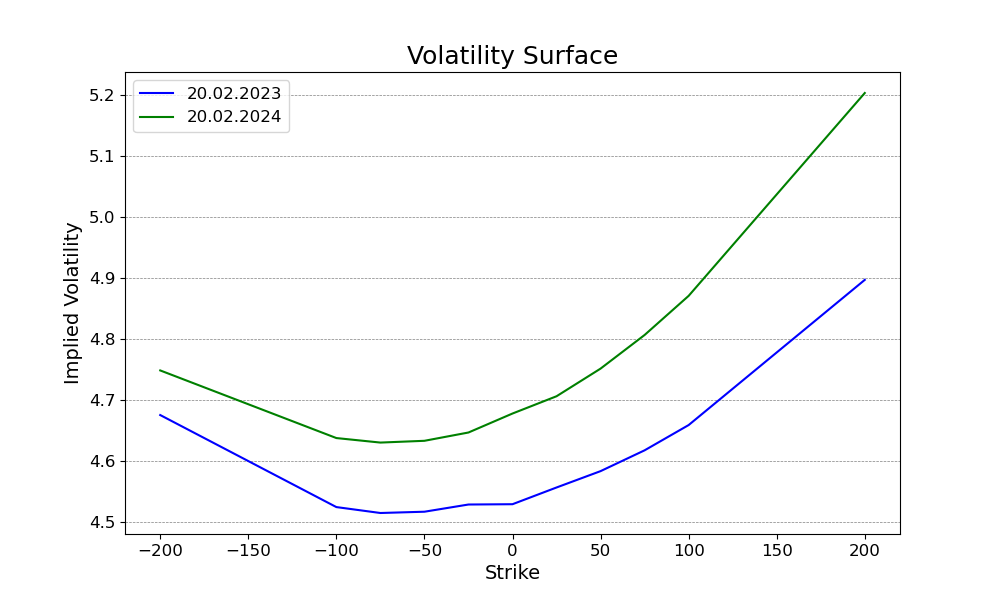
\includegraphics[width=\linewidth]{/Users/nannaingemannohrt/Desktop/master_thesis/main/plots/10Y12Y.png}
        \caption{EUR swaption 10Y12Y}
        \label{fig:10Y12Y}
    \end{minipage}\hfill 
    \begin{minipage}{0.5\textwidth}
        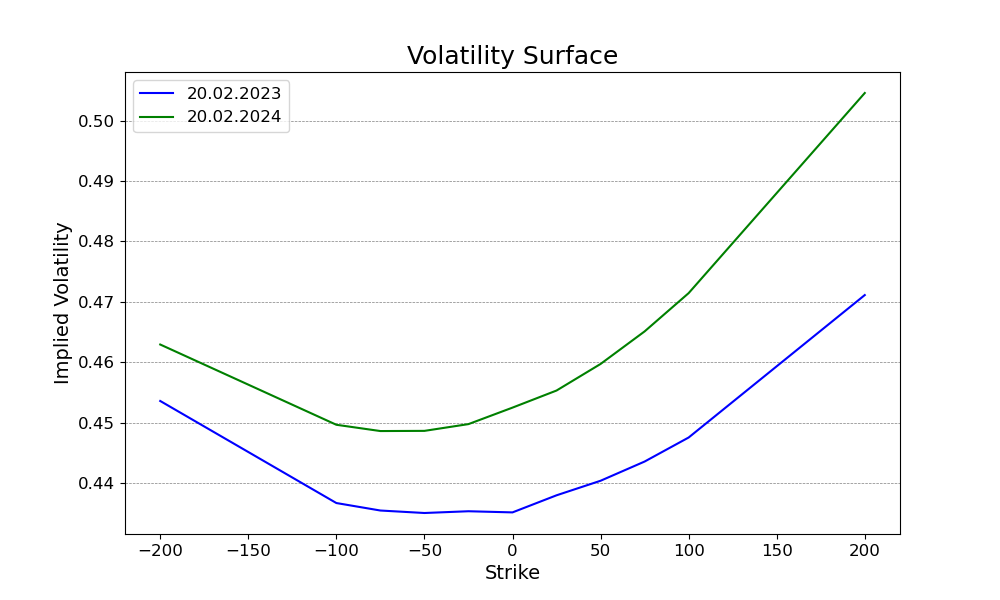
\includegraphics[width=\linewidth]{/Users/nannaingemannohrt/Desktop/master_thesis/main/plots/10Y15Y.png}
        \caption{EUR swaption 10Y15Y}
        \label{fig:10Y15Y}
    \end{minipage}

    \centering
    \begin{minipage}{0.5\textwidth}
        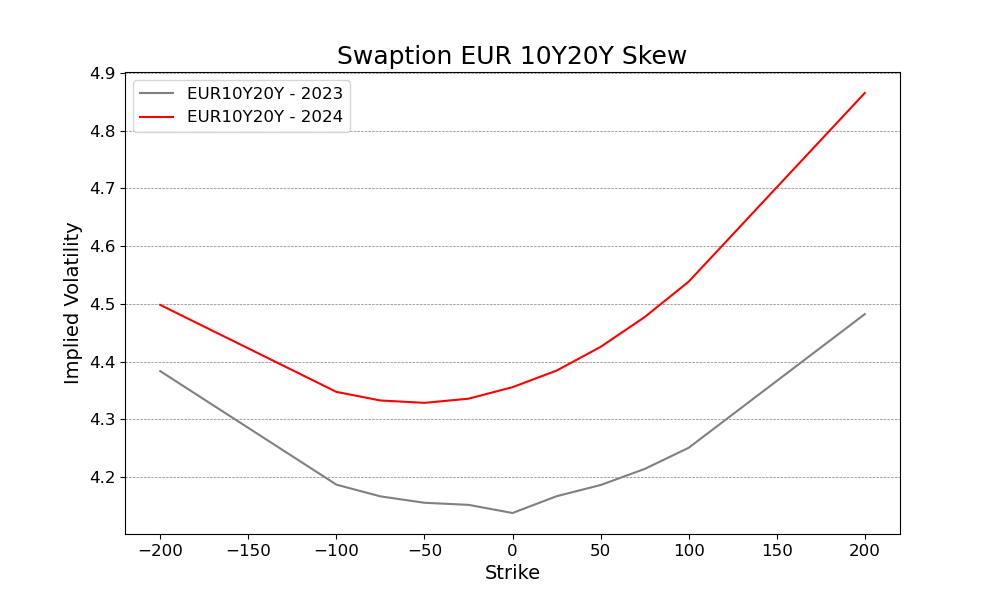
\includegraphics[width=\linewidth]{/Users/nannaingemannohrt/Desktop/master_thesis/main/plots/10Y20Y.png}
        \caption{EUR swaption 10Y20Y}
        \label{fig:10Y20Y}
    \end{minipage}\hfill 
    \begin{minipage}{0.5\textwidth}
        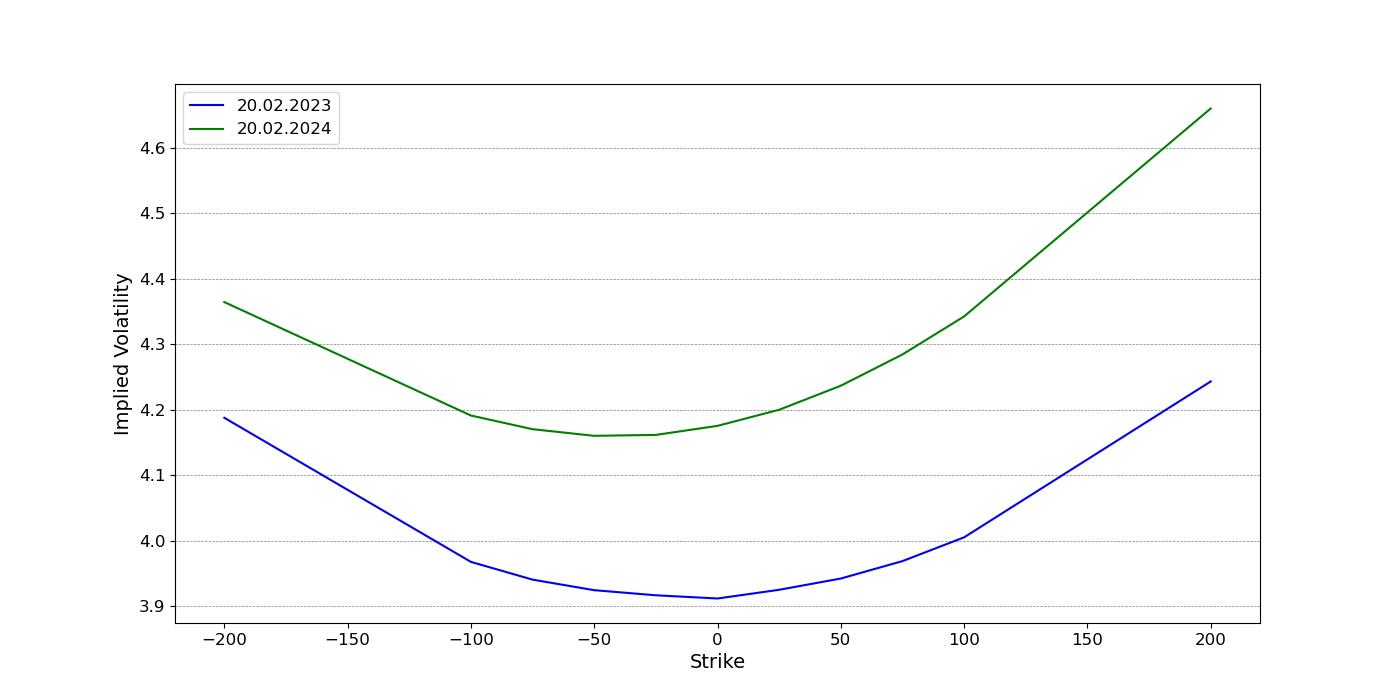
\includegraphics[width=\linewidth]{/Users/nannaingemannohrt/Desktop/master_thesis/main/plots/10Y30Y.png}
        \caption{EUR swaption 10Y30Y}
        \label{fig:10Y30Y}
    \end{minipage}
\end{figure}


    